\chapter{Réalisation}
	\section{Introduction}
		Dans ce chapitre, nous passerons en revu la réalisation des termes évoqués tout au longs les lignes précédentes. Nous aborderons égalements les difficultés techniques rencontrées durant le stage.
	\section{Création d'un utilisateur}
	La gestion des utilisateurs est une fonctionnalité indispensable dans la création d'un back office. Dans le système mis en place, pour que les données des utilisateurs soient prises en compte, plusieurs phases de vérifications doivent être éffectuées. Lorsque l'utilisateur renseigne ses informations, la phase de validation de données est déclenchée. Si les données ne sont pas valides alors un ensemble de message d'erreurs est renvoyé à ce dernier.\\
	Dans le cas contraire, un mail de vérification est envoyé à l'utilisateur pour comfirmer son adresse mail.\\
	Tout ce processus peut être inité par deux méthodes: \textbf{Commande symfony} et \textbf{le back office}.\\
	
		\textbf{Depuis une commande Symfony: } L'accès au back office requière le compte d'un utilisateur pré-enregistré dans la base de données.
			Pour un projet initialisé, il n'existe aucun utilisateur crée dans la base de données ce qui peut être problématique. Ainsi la création d'une commande symfony de créer le compte d'un utilisateur sans passer par une interface graphique.\\
			
		\textbf{Depuis le back-office: } En plus d'une commande Symfony, une interface graphique permet à un administrateur.
	\section{Authenfication}
		L'authentification est une couche de sécurité mise en place pour accéder aux fonctionnalités réservées aux administrateurs. Pour y accéder, l’utilisateur doit avoir un compte déjà créer par un administrateur au préalable.
		\begin{center}
			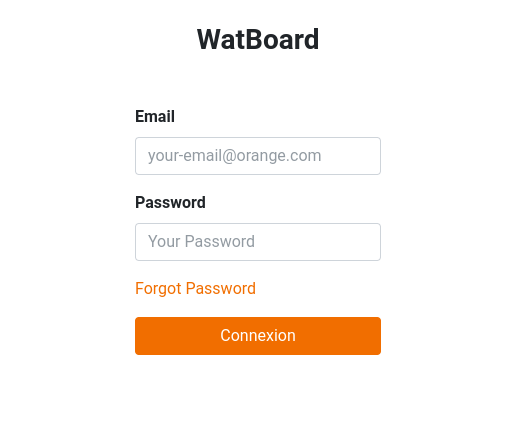
\includegraphics[scale=0.4]{chap_3/authen.png}
			\captionof{figure}{Authenfication}
			\label{Authenfication}
		\end{center}
	\section{API de récupération des fichiers de rapports}
		Les rapports de qualité de code, tests, sécurités sont générés depuis GitLab CI/CD. 
		Ces rapports sont appelés artefacts dans le contexte d’intégration continue. Un pipeline regroupe un ensemble de stage destiné à faire des tâches spécifiques (appelée jobs). Ainsi, dans notre système d’intégration continue mise en place, nous avons plusieurs stages permettant d’analyser le code écrit par les développeurs tels que : Quality, tests, security, etc.  En fonction de chaque stage, il existe des outils appropriés à effectuer les tâches qu’il faut. Par exemple   PHPQA pour l’analyse de la qualité de code, Codeception pour les tests, Trivy pour la vérification de la sécurité des packages.\\
		À la fin de chaque stage, les fichiers de rapports sont générés. Ces fichiers de rapports sont envoyés par API à notre application qui aura pour tâches:
		\begin{itemize}
			\item Stocker les données récupérer dans ces fichiers et les stocker dans une base de données.
			\item Afficher les diagrammes à travers ces données stockées.
		\end{itemize}  
		
	\section{Dashboard}
		\subsection{Récapitulatif de l'etat d'un projet}
			Le récapitulatif global d’un projet consiste à avoir un aperçu global sur l’état d’un projet. On pourrait y voir les informations suivantes :\\
			\begin{itemize}
				\item \textbf{Le nombre de builds} : Correspond au nombre de fois qu’un projet a été déployé dans le pipeline.
				\item \textbf{Le nombre d’erreurs} : Correspond au nombre d’erreurs repéré dans tous les rapports.
				\item \textbf{Le nombre de warnings} : Correspond au nombre d’avertissements repéré dans tous les rapports.
				\item  \textbf{La tendance} : Est une fonctionnalité qui consiste à analyser l’état d’un projet sur certain nombre de builds (cinq, dix, ou plus). En fonction de ces analyses, on peut en déduire plusieurs états : 
					\begin{itemize}
						\item \textbf{Soleil} : Lorsqu’on constate une évolution de la qualité de code sur les dix derniers builds.
						\item \textbf{Nuageux} : Lorsqu’on constate une évolution sur les cinq derniers builds.
						\item \textbf{Pluie} : Lorsque les deux cas ne sont pas respectés.
					\end{itemize}
			\end{itemize}
		\begin{center}
			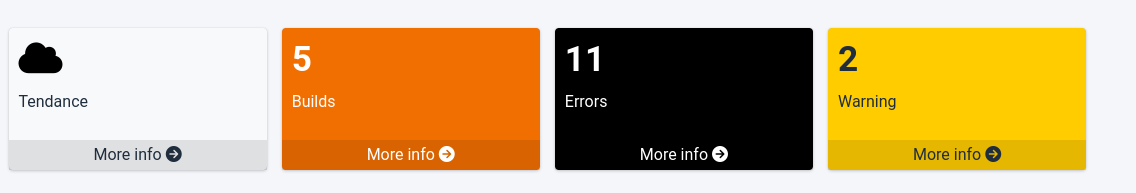
\includegraphics[scale=0.4]{chap_3/recapt.png}
			\captionof{figure}{Recaptulatif}
			\label{Recaptulatif}
		\end{center}
		\subsection{Diagrammes}
			\subsubsection{Build}
				Le diagramme de builds est un graphique permettant d'afficher l'évolution d'un projet en fonction des issues (erreurs + warnings) récupérés dans les fichiers de rapports.
				Un coup d'œil sur ce diagramme permet de savoir si un projet est en régression ou non.
				\begin{center}
					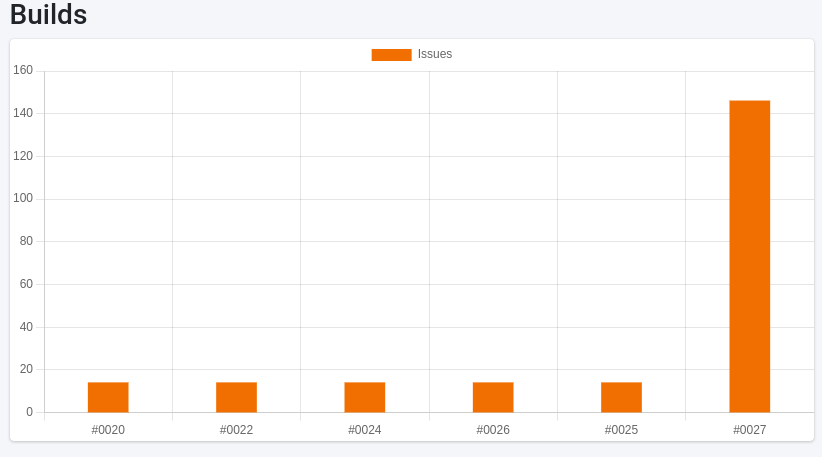
\includegraphics[scale=0.4]{chap_4/graphique-build.png}
					\captionof{figure}{Diagramme - builds}
					\label{Graphique builds}
				\end{center}
			\subsubsection{Outils}
			En plus de la tendance, le diagramme d'un outil permet de mettre en lumière l'évolution d'un projet vis à vis de l'utilisation cet outil à travers un diagramme en lignes.
				\begin{center}
					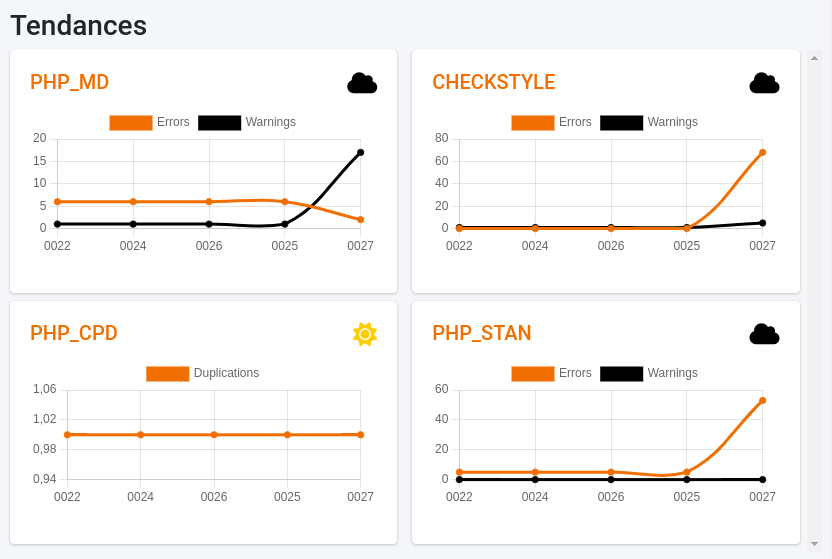
\includegraphics[scale=0.5]{chap_4/tendance-outils.png}
					\captionof{figure}{Diagramme - outils}
					\label{Diagramme - outils}
				\end{center}
		\subsection{Tableau de builds}
		Le tableau de build permet d'afficher l'historique des builds d'un projet et leurs issues. Il est possible d'interagir avec ce tableau pour afficher la répartition de ces issues par outils de qualité de code.\\
		\begin{center}
			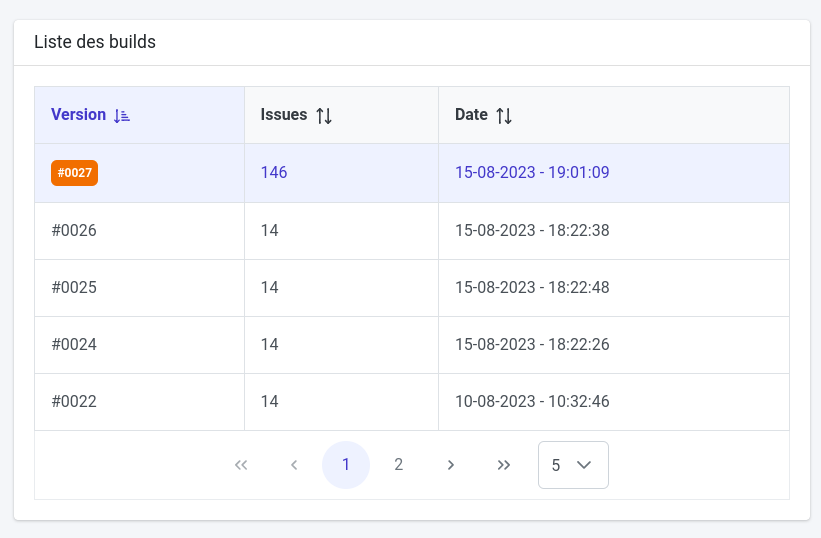
\includegraphics[scale=0.5]{chap_4/tableau-builds.png}
			\captionof{figure}{Tableau - build}
			\label{Tableau - builds}
		\end{center}
		Un clique sur une ligne du tableau permet d'afficher un digramme en camembert montrant la répartion des issues à travers les outils utilisés.
		\begin{center}
			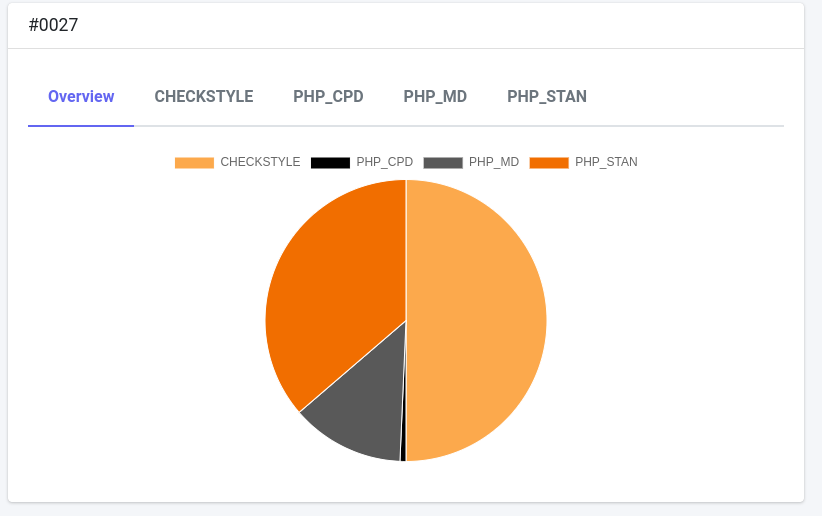
\includegraphics[scale=0.5]{chap_4/repartion-outils.png}
			\captionof{figure}{Repartition - outils}
			\label{Repartition - outils}
		\end{center}